
\documentclass[11pt]{article}

\usepackage{amsmath} %import amsmath for align command
\usepackage{cite} %import package for using bibtex bibliography
\usepackage{graphicx} %import package for inserting figures from image files
\usepackage{mathtools} %import package for using certain symbols such as eq. arrows
\usepackage{tikz} %import package for creating figures
\usepackage{booktabs}
\usepackage{siunitx}
\usepackage[T1]{fontenc}
\usepackage[font=small,skip=0pt]{caption}


\usepackage{placeins}
\usepackage{array}
\newcolumntype{P}[1]{>{\centering\arraybackslash}p{#1}}

\usepackage[nodisplayskipstretch]{setspace}


\usepackage{titlesec}
\titlespacing{\section}{0pt}{0.8\baselineskip}{0.8\baselineskip}
\titlespacing{\subsection}{0pt}{0.675\baselineskip}{0.675\baselineskip}
\setlength{\abovecaptionskip}{2pt plus 2pt minus 5pt}

% for referencing links
\usepackage{hyperref}
\hypersetup{
	colorlinks=true,
	linkcolor=blue,
	filecolor=magenta,
	urlcolor=cyan,
}

% \usepackage{apacite}

\usepackage{algorithm}
\usepackage[noend]{algpseudocode}
\usepackage{textcomp}
\usepackage{subcaption}

%change default margins
\setlength{\topmargin}{-.75in}
\setlength{\textheight}{9.5in}

\setlength{\oddsidemargin}{0in}
\setlength{\evensidemargin}{0in}
\setlength{\textwidth}{6.6in}

\graphicspath{{aima/images/}}

\newcommand{\urlNewWindow}[1]{\href[pdfnewwindow=true]{#1}{\nolinkurl{#1}}}
\newcommand{\problemone}{grid world problem}
\newcommand{\Problemone}{grid world problem}
\newcommand{\problemtwo}{choice suggestion problem}
\newcommand{\Problemtwo}{choice suggestion problem}
\newcommand{\expnumber}[2]{{#1}\mathrm{e}{#2}}

\begin{document}

%create title
\title{Deep Reinforcement Learning Nanodegree\\
	   Project 2 -- Continuous Control Report}
\author{\vspace{-1mm}Chris Cadonic\\
chriscadonic@gmail.com}
\maketitle
\vspace{-1.5em}

\section{Introduction}

\subsection{Environment Overview}

\FloatBarrier

\begin{figure}[!ht]
	\centering
	%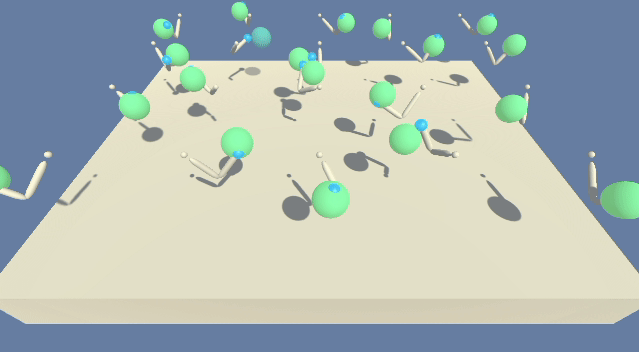
\includegraphics[width=0.75\linewidth]{images/example-env-image.png}
	\caption{A snapshot of the continuous control Unity-ML Reacher environment.}
	\label{fig:example-game-image}
\end{figure}

\FloatBarrier

\section{Approach}

\subsection{D4PG}

\subsection{Implementation}

 \FloatBarrier
 
 \begin{figure}[!ht]
 	\centering
 	%\includegraphics[width=\linewidth]{images/nn-architecture.png}
 	%\caption{The 8-layer MLP used in the DQN algorithm.}
 	\label{fig:nn-architecture}
 \end{figure}
 
 \FloatBarrier
 
\FloatBarrier

\begin{table}[!ht]
	\centering
	\begin{tabular}{ c | c }
	\textbf{hyperparameter} & \textbf{values} \\
	\hline
	$\epsilon_{decay}$ & $[0.99, 0.996, 0.999, 0.9999, 0.99999]$ \\
	$\alpha$ & $[0.00005, 0.0001, 0.0005, 0.001, 0.005]$ \\
	$\tau$ & $[0.005, 0.01, 0.1]$ \\
	$\gamma$ & $[0.8, 0.9, 0.95, 0.99]$ \\
	\hline
	\end{tabular}
	\caption{Hyperparameters experimented with to train an agent using DQN.}
	\label{tbl:parameters}
\end{table}

\FloatBarrier

\section{Results and Discussion}

\subsection{Learning Performance}

\FloatBarrier

\begin{figure}[!ht]
	\centering
	%\includegraphics[width=0.9\linewidth]{images/d4pg-results.png}
	\caption{}
	\label{fig:d4pg-results}
\end{figure}

\FloatBarrier

\begin{itemize}
	\item $\epsilon_{decay} = 0.996$,
	\item $\alpha = 0.001$,
	\item $\tau = 0.01$,
	\item $\gamma = 0.99$.
\end{itemize}

\subsection{Next Steps}

\section{Conclusion}

\bibliographystyle{unsrt}
\bibliography{refs}
% \begin{thebibliography}{9}
% \bibitem{littman}
% Leslie~Pack Kaelbling, Michael~L Littman, and Andrew~W Moore.
% \newblock Reinforcement learning: A survey.
% \newblock {\em Journal of artificial intelligence research}, 4:237--285, 1996.
% \end{thebibliography}

\end{document}
